\chapter{THE REVERSE-MAPPING PROBLEM}
\thispagestyle{plain}

\label{ReverseMapping}

The reverse-mapping problem is the problem of defining a function $f^{-1}$ that maps a system-level configuration $\mathbf y$ onto a solution space $\hat{\mathbf S}$ that represents all possible configurations that would cause the system to exhibit $\mathbf y$:
   \[ f^{-1}(\mathbf y) \rightarrow \hat{\mathbf S}. \]
Every configuration $\hat {\mathbf x} \in \hat {\mathbf S}$ should satisfy the constraint $f(\hat{\mathbf x}) \approx \mathbf y$, where $f$ is the forward mapping.
That is, $\hat{\mathbf S}$ is the set of all the points that would predict $\mathbf y$ in the forward mapping.

The major difficulty in solving the reverse-mapping problem is that the mapping is one-to-many because the forward mapping is built with regression (many-to-one).
Therefore, querying a reverse mapping returns a solution space, not a singular solution.
For this reason, \fw strives to return the \textit{space of configurations} that will exhibit a given system-level property in an ABM, not individual configurations.

This general method of developing a reverse mapping can be contrasted with optimization methods (see Section \ref{sec:invfm}).
Finding a set of configuration parameters that satisfies a system-level property, by definition, is an optimization problem.
However, instead of a single point being returned as in most optimization methods, a reverse mapping returns the space of all points that would satisfy the configuration.
This approach has a number of benefits, such as being able to visualize and inspect the entire solution space.
Analysis of how the solution space changes with respect to the configuration parameters can be performed.
Different solutions that produce similar results can be selected from a number of good solutions based on some exterior preference on configurations.
That is, although all points in a solution space should be satisfactory, some points may be more desirable for a number of reasons, such as points with lower expected variance.

In this chapter, I give details of how \fw provides one solutions to this problem then discusses actual implementations of the solution.
Throughout this chapter, I use the NetLogo Fires ABM\footnote{Details of the Fires model is discussed in Section \ref{sec:Fires}.} as an example.
The Fires domain is simple and has solution spaces that are easy to visualize.
Other domains, such as Wolf Sheep Predation, have too many dimensions to make graphing feasible.
The arguments made with the aid of the Fires domain scale to larger dimensions.



\section{\fw Approach: simplicial Complex Inversion}
The first \fw reverse-mapping approach is a novel approach I developed, named \textit{simplicial Complex Inversion} (SCI).
A simplicial complex is a set of adjacent simplexes (multi-dimensional triangles) that partition the space.
In abstract terms, SCI builds an invertible approximation of the forward mapping in the form of a simplicial complex.
This approach is used because regression is not easily invertible.
I have found that inverting even the simplest approaches such as K-nearest neighbor and LOESS are either difficult to implement or computationally expensive (Section \ref{sec:functional}).
By approximating a representation of the forward mapping that is invertible, solving the reverse-mapping problem becomes computationally tractable.
These direct inversion approaches are generally not preferred over SCI, since they are dependent on the forward mapping approach used and SCI is applicable to any forward-mapping technique.
\textit{SCI is building an invertible approximation of a trained forward mapping.}
This is in contrast to building a reverse mapping directly from the training data.

As with the forward-mapping solution, the system-level property $\mathbf y$ is split into subspaces to simplify the problem:
\[ \mathbf y = \{y_0, y_1, \ldots, y_{|\mathbf y|}\}. \]
The solution space is split up in a similar manner:
\[ \hat{\mathbf S} = \{\hat S_0, \hat S_1, \ldots, \hat S_{|\mathbf S|}\}. \]
By performing this split, each forward mapping can be inverted independently:
\[ f^{-1}_i(y_i) \rightarrow \hat S_i. \]

Recombining the individual $\hat S_i$ into $\hat{\mathbf S}$ is not as simple as recombining individual $\hat y_i$ into $\hat{\mathbf y}$ in the forward-mapping solution.
Since each solution space represents which configurations satisfy a particular system-level requirement, the solution space $\hat{\mathbf S}$ is the intersection of all of these spaces:
\[ \hat{\mathbf S} = \hat S_0 \cap \hat S_1 \cap \ldots \cap \hat S_{|\mathbf S|}.\]
All points at the intersection of these spaces should satisfy all system-level properties at once.

simplicial Complex Inversion has three phases.
First, regression is used to infer the system-level property values for several ``knots"\footnote{The term ``knot" is taken from Multilinear Interpolation \cite{davies1997multidimensional} (section \ref{sec:multilinear}).} in the configuration space.
The locations of these knots are used to segregate the configuration space into a number of simplexes.
This segregated configuration space is referred to as a \textit{simplicial complex} \cite{munkres1993simplicial}.
Next, the intersection between each of these simplexes and a plane representing the target system-level property is found.
That is, SCI derives the equation of the hyperplane through each simplex that satisfies the target system-level property.
A piecewise linear represention of the configurations that would satisfy the target system-level property is constructed from all the intersections.
Figure \ref{fig:ISFlow} illustrates the SCI process; the rest of this subsection dscusses these steps in detail.

\begin{figure}[ht]
\centering
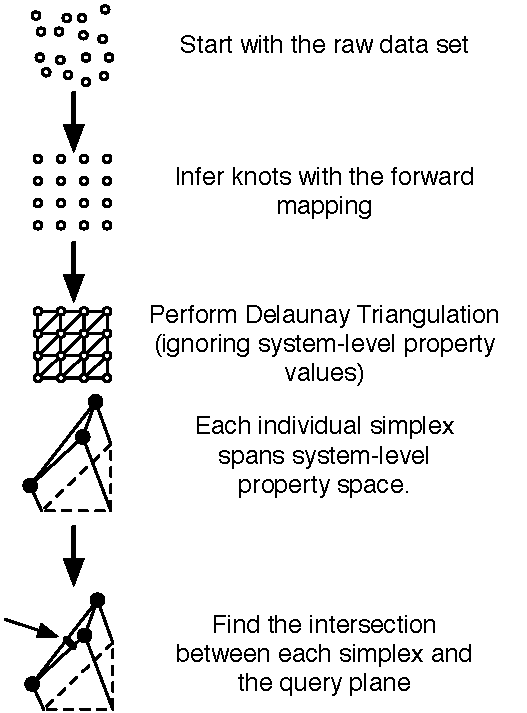
\includegraphics[scale=1]{images/ISflow.pdf}
\caption{The flow of stages in the simplicial Complex Inversion approach to the reverse-mapping problem in a two-dimensional configuration space.}
\label{fig:ISFlow}
\end{figure}

I claim that SCI is a general approach to the reverse-mapping problem that is applicable in all domains in which the forward-mapping problem is solved accurately.
Also, SCI provides more useful information than optimization, since SCI returns the \textit{set} of all configurations.
These hyperplanes give a more continuous and complete view of the nature of a specific system-level property value than individual points.




\begin{figure}[ht]
\centering
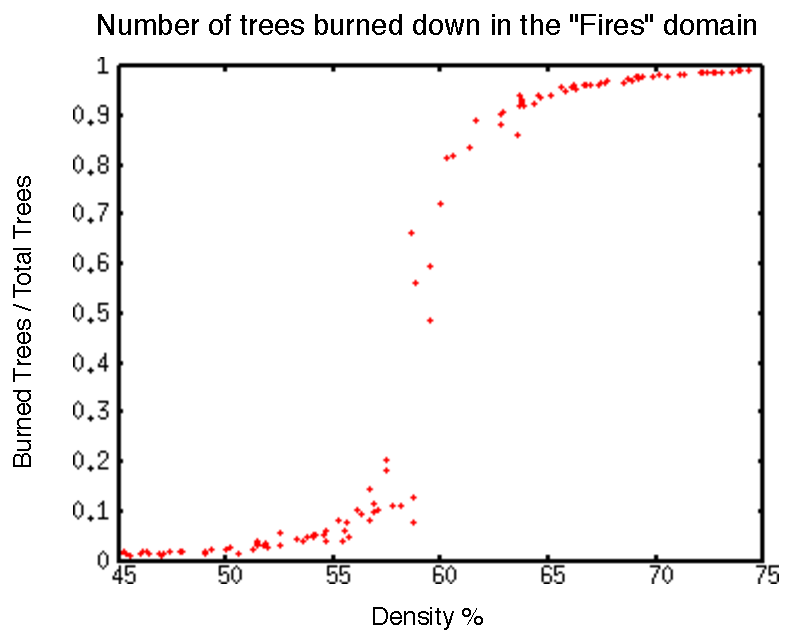
\includegraphics[scale=.66666667]{images/rii0.pdf}
\caption{The raw data set, containing 120 points, from the Fires domain.}
\label{fig:rii0}
\end{figure}

\begin{figure}[ht]
\centering
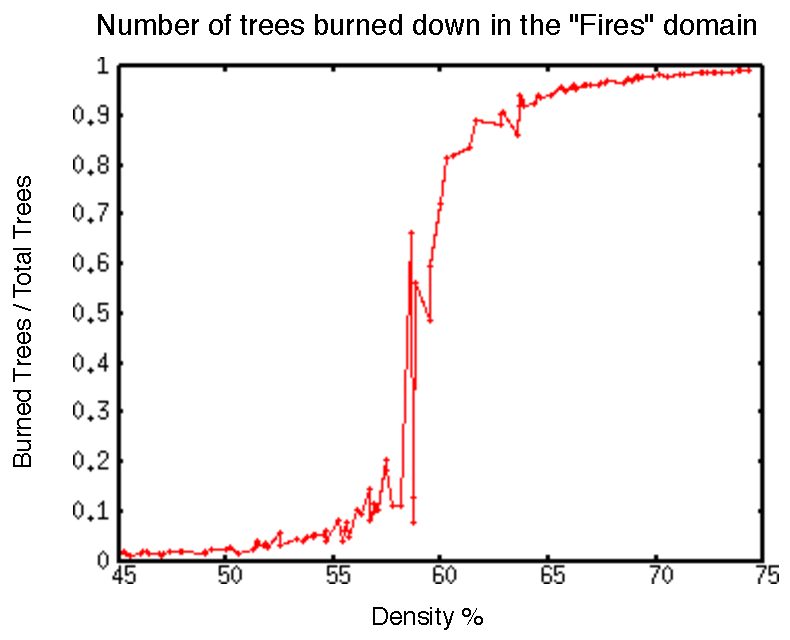
\includegraphics[scale=.66666667]{images/rii1.pdf}
\caption{Linear interpolation performed on the raw data set (see Figure \ref{fig:rii0}) from the Fires domain.}
\label{fig:rii1}
\end{figure}

\subsection{Segregating the Configuration Space}
The reason for using regression as the first step is that the raw data in many ABMs will exhibit variance.
For example, raw data from the Fires ABM is shown in Figure \ref{fig:rii0}.
If this data were to be used with interpolation, the curve for the behavior space would be very erratic.
This is a problem for SCI because erratic curves will result in a number of inaccurate intersections.
A linear interpolation performed on the raw Fires data to generate a behavior space curve is shown in Figure \ref{fig:rii1}.
From this figure, the curve appears very erratic and would provide poor results with SCI.


The behavior space is naturally much smoother when mapped to the regression space.
The first step of SCI is to use the forward mapping (i.e., regression) to infer knots in the space, which are evenly distributed across the range of sampled values.
The granularity of the knots is specified by the user.
These knots cover the space and provide reference points for the interpolation.
To generate these points, the forward mapping is queried by passing a complete vector of configuration parameters.
An inferred system-level property value is returned.
Each data knot in an $n$-dimensional\footnote{$n$ refers to the dimensionality of the configuration space for the rest of this chapter.}  configuration space is represented by a vector of configuration space parameter values ($\mathbf x$) and the system-level property value ($y$):
\[<x_1, x_2, ..., x_n, y>.\]

The configuration space is then segregated with Delaunay triangulation \cite{delaunay1934sphere} into adjacent simplexes (simplicial complex).
These simplexes have $n + 1$ corners (e.g., they are triangles if $n=2$ and lines if $n=1$) and spans $(n+1)$-dimensional space.
Note that the behavior space resides in $(n+1)$-dimensional space, but the simplexes are $n$-dimensional objects (e.g., a tetrahedron in four-dimensional space if $n=3$ or a line segment in two-dimensional space if $n=1$).
This is because the system-level property $y$ is not taken into consideration for the the Delaunay triangulation.
The relationships between these objects' dimensionality and different dimensional configuration spaces are outlined in Table \ref{table:dims}.
For example, in the Fires ABM (1-dimensional configuration space), the space is segregated into line segments that reside in two-dimensional space.

\begin{table}[ht]
  \caption{Dimensionality of Objects for Simplex Inversion}
  \centering
  \begin{tabular}{c c c c}
    \hline \hline
    Configuration Space & Behavior Space & Simplex & Intersection \\
    Dimensionality      & Dimensionality &         &  \\
    \hline
    1 & 2 & line & point \\
    2 & 3 & triangle & line \\
    3 & 4 & tetrahedron & plane \\
    4 & 5 & pentachoron & 3D hyperplane \\
    5 & 6 & 5-simplex & 4D hyperplane \\
    $\vdots$ & $\vdots$ & $\vdots$ & $\vdots$ \\
    $n$ & $n + 1$ & $n$-simplex & ($n-1$)D hyperplane \\
    \hline
  \end{tabular}
  \label{table:dims}
\end{table}

%Delaunay triangulation is used to segregate the space.
If the configuration points were randomly scattered, a standard algorithm for computing the Delaunay triangulation could be used.
However, since SCI controls how configuration points are distributed, it can organize the points in such a way that a solution to the Delaunay triangulation can be computed implicitly.
In general, SCI will evenly space the sample points as a grid and split each hypercube into two simplexes.
The Delaunay triangulation is trivial to compute with points organized in this way.
For example, in Figure \ref{fig:ISFlow}, the space is segregated into a number of adjacent triangles that satisfy the requirements for being a Delaunay triangulation.
To segregate the space into a Delaunay triangulation from a regular grid, each hypercube is split into two simplexes.
The two simplexes are defined as the simplex defined with all the corners except for the corner closest to the origin, and as the simplex defined with all the corners except for the corner furthest from the origin.
For example, with a square, two triangles are formed with two opposite corners as the right angles for their respective triangles.

The equations of the simplexes can be defined in terms of the hyperplane in which they reside.
The $n+1$ points define a $n$-dimensional hyperplane.
If a point is within all the facets and lies on the hyperplane, the point is on the simplex.
For example, in the Fires ABM, the two points defining a line segment reside on a line that extends infinitely in both directions.
Meanwhile, the facets are defined by the points individually.
If a behavior space point lies on the line and resides between the two facet points, the point is a plausible configration that would generate the desired system-level behavior.
This explanation expands to two-dimensional configuration spaces, which have triangles as simplexes and line as facets.
If a point lies on the plane defined by the the points, and is within the boundaries of the line segment facets, the point is realistic.


\begin{figure}[ht]
\centering
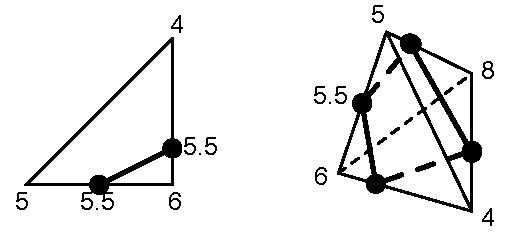
\includegraphics[scale=1]{images/simint.pdf}
\caption{A triangle from a two-dimensional configuration space (left) and a tetrahedron from a three-dimensional configuration space (right) are intersected with the plane $y=5.5$. The $y$-values for each corner are given.}
\label{fig:simint}
\end{figure}

\subsection{Simplex Intersection}
Recall that the final goal of this process is to find the equation of the intersection between all the simplexes and a system-level property hyperplane.
Therefore, no complicated technique needs to be performed to calculate the actual equation of the simplex or the facets.
Edge intersections are used to approximate the intersection through the simplex.
The process to find the intersection between the system-level property hyperplane and a simplex is as follows:
\begin{enumerate}
   \item Pair off each corner with every other corner, in every possible combination. These point pairs define the edges of the simplex.
   \item Determine which edges intersect with the hyperplane. An edge intersects with the hyperplane if the target system-level property value  is between the $y$-values for the two points that define the edge. From the intermediate-value theorem, the plane must intersect with this line segment at some point, at least once.
   \item Use linear interpolation to determine at which point on the edge line segment on which the intersection occurs.
For example, suppose that the corners have $y$-values of 2 and 4 and the target system-level property value is 3.
The location of the intersection is halfway between the corners.
   \item The set of all edge intersection points lies on the hyperplane that intersects the simplex. Use these points to define the intersecting hyperplane.
\end{enumerate}
This approach circumvents the need for modeling the actual simplexes as equations, which can be challenging to implement.
Two illustrative examples of this intersection method are shown in Figure \ref{fig:simint}.
In the example on the right-hand side in Figure \ref{fig:simint}, the two-dimensional plane intersects the tetrahedron in four places.
However, only three of these points are needed to define the plane because the fourth point is coplanar and thus redundant.
This illustrates the fact that not every edge has to be checked for intersection, only enough points to define the intersecting hyperplane.
Since the intersecting hyperplane is $(n-1)$D, $n$ points are needed.
SCI uses the following standard representation for a plane, where $\mathbf C$ is a vector of constants and $\mathbf x$ is the vector of configuration parameters and system-level properties:
\[\mathbf C \cdot \mathbf x + D = 0\]
\[C_0 x_0 + C_1 x_0 + ... + C_n x_n + C_{n+1} x_{n+1} + D = 0. \]

This approach is very general and will work in most cases; however, when the plane intersects with either a corner point or an edge only, no plane can be defined because not enough non-colinear points can be found.
To circumvent this problem, SCI considers the boundaries of the simplex not to be part of the simplex.
Thus, a point that intersects with only the corner or an edge will not be considered in the final piecewise intersection.

\subsection{Recombination of Solution Spaces}

Once solution spaces have been found for each of the desired system-level properties, they are recombined into one solution space.
This final solution space will be a piecewise hyperplane function, consisting of points that exhibit the specified system-level property values.
Since the individual reverse mappings are hyperplanes, the recombination is the intersection of all these hyperplanes.


\begin{figure}[ht]
\centering
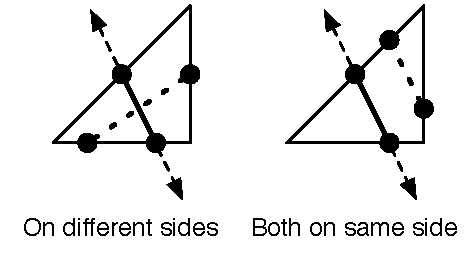
\includegraphics[scale=1]{images/intcheck.pdf}
\caption{Illustration of two recombination scenarios: intersecting (left) and not intersecting (right).}
\label{fig:intcheck}
\end{figure}


First, SCI verifies if the hyperplanes intersect within the simplex.
Two hyperplanes intersect if the points on one hyperplane are separated by the other hyperplane.
If the points are separated, then there must be an intersection.
An illustration of points being separated by a hyperplane, and not, is shown in Figure \ref{fig:intcheck}.
This intersection check is performed by plugging in values for the edge intersections of one hyperplane into the equation of other hyperplane.
Then, the nature of the inequality (greater-than or less-than) for each point specifies which side the edge intersection is on.
If one point is on the other side of another point, the planes intersect.
This calculation is easy to perform since SCI has the edge intersection points and the equation of the hyperplanes already computed.
Also, this process can be repeated for any number of hyperplanes by performing this test for each possible pair of hyperplanes.
However, it may be the case that the hyperplanes do not intersect in the same places, even if all of the  hyperplanes intersect, pairwise.


To find the intersection, a system of linear equations is set up in matrix form:
\[  \left[ \begin{array}{ccccc}
C_{0,0} & C_{0, 1} & ... & C_{0,n+1} & D_0 \\
C_{1,0} & C_{1, 1} & ... & C_{1,n+1} & D_1 \\
\vdots  & \vdots   & \vdots & \vdots & \vdots \\
C_{m,0} & C_{m, 1} & ... & C_{m, n+1} & D_m \end{array} \right]
\left[ \begin{array}{c}
x_0 \\
x_1 \\
\vdots \\
x_{n+1} \end{array} \right] = \mathbf 0
\] 
To solve this system of equations, SCI reduces the coefficient matrix to reduced row echelon form (RREF).
What remains is a system of reduced linear equations that are more concise in defining the intersection.
From the check performed as the first step, any intersections returned by the solution of this system of equations is guaranteed to be within the simplex.


The RREF can reveal that the system is either overspecified or underspecified.
A system of equations is overspecified if there is a row in RREF that is all zeros, except for the last column value $D \neq 0$:
\[ \left[ \begin{array}{ccccc} 0 & 0 & ... & 0 & D \end{array} \right]. \]
This row translates to $0 = D$, which is not true.
That is, there is no possible configuration of $\mathbf x$ that will satisfy this specific equation.
Thus, the set of system-level properties the user has provided is not able to be created with this ABM.
This situation is typical if the user has specified too many requirements of the system-level properties.
In this case, the user should remove some less important system-level property requirements and allow the system to suggest values for them.

RREF reveals that the system is underspecified if there are any rows with multiple non-zero values in it, other than $D$. For example, consider the row pulled from a matrix in RREF:
\[ \left[ \begin{array}{ccccc} 0 & 1 & 2 & 0 & 5 \end{array} \right]. \]
This row translates to $x_1 + 2x_2 = 5$.
Therefore, $x_1$ and $x_2$ are free variables, but are still constrained by this equation.
An infinite number of solutions can satisfy the system-level properties in this case.
This is not a problem like being overspecified, since there are a number of possible solutions available to the user.


\subsection{Granularity}
\label{subsec:granularity}

SCI can be configured by adjusting the granularity of the knots.
SCI approximates an invertible continuous representation of the forward mapping.
Therefore, as the granularity of SCI increases, it models the forward mapping more accurately.
Thus, the granularity should be as high as computationally acceptable.

Granularity can be adjusted dynamically on a query-by-query basis.
Individual simplexes may be separated into several subsimplexes.
These new simplexes are composed of the original simplex's corners, in addition to new corners.
The new corners have their system-level property value inferred from the forward mapping.
Once these new simplexes have been formed, nothing special has to be performed to accommodate them in the general SCI algorithm.
In addition, even if the granularity has been increased for a specific query, the finer-grained simplexes can remain to increase the accuracy of future queries.

Dynamic adjustment of the granularity process can be performed automatically to increase the accuracy of simplexes that contain significant amounts of variability between the system-level property values at the corners.
Increasing the granularity will reduce the variance, since points closer to one another will have increasingly similar values.

The effect of the granularity on accuracy is dependent on the nature of the forward-mapping regression method used.
If the forward-mapping produces overfit or otherwise inaccurate predictions, the predictions that the reverse mapping produce will be inaccurate as well.
This difficulty should be dealt with in the forward-mapping solving step, not the reverse-mapping solving step.
This is because the purpose of SCI is to model the forward-mapping, not the domain.

An empirical analysis of the relationship between granularity and accuracy is provided in Chapter \ref{Results}.
The accuracy is measured as the approximate total difference between the continuous forward-mapping function and the continuous simplicial complex.
In addition, suggestions made from SCI are validated against an actual system run of the target ABM.
The error between the desired system-level property values and the actual system-level property values are measured.
This measurement is redundant, since the error between the actual run and the reverse-mapping solution should be the sum of the forward mapping error and the reverse mapping error (in respect to the forward mapping).


\subsection{Example: Fires ABM}

Figure \ref{fig:rii} illustrates the progression of SCI from step to step when used for the Fires ABM.
First, the forward-mapping problem is solved, with any regression method.
Then, the knots are formed in evenly spaced intervals: in this case, intervals of 1\% tree density (see top right image in Figure \ref{fig:rii}).
The simplexes in the case of the Fires ABM are line segments, since the configuration space is one-dimensional.
Therefore, linear interpolation between the points produces the simplexes (see bottom left image in Figure \ref{fig:rii}).
Each segment is also the only edge of the simplex.

\begin{figure}[ht]
\centering
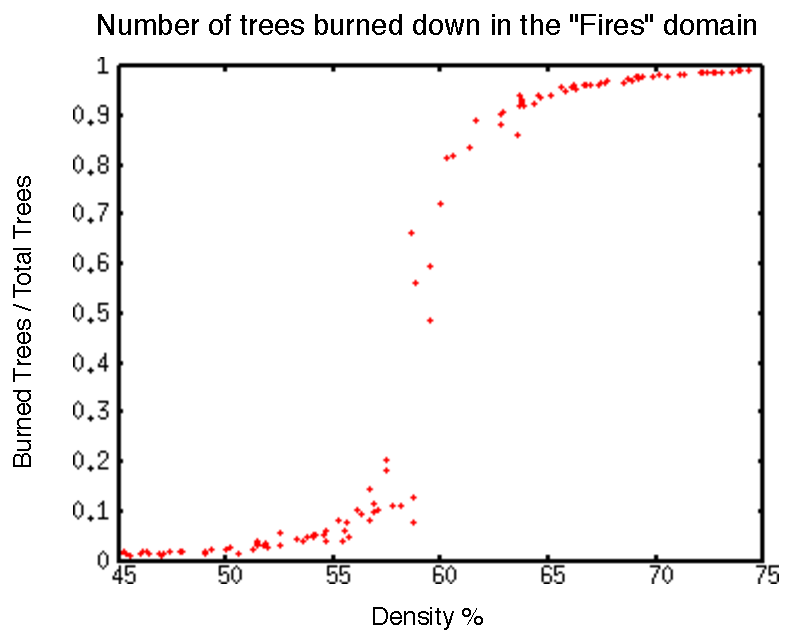
\includegraphics[scale=.5]{images/rii0.pdf}
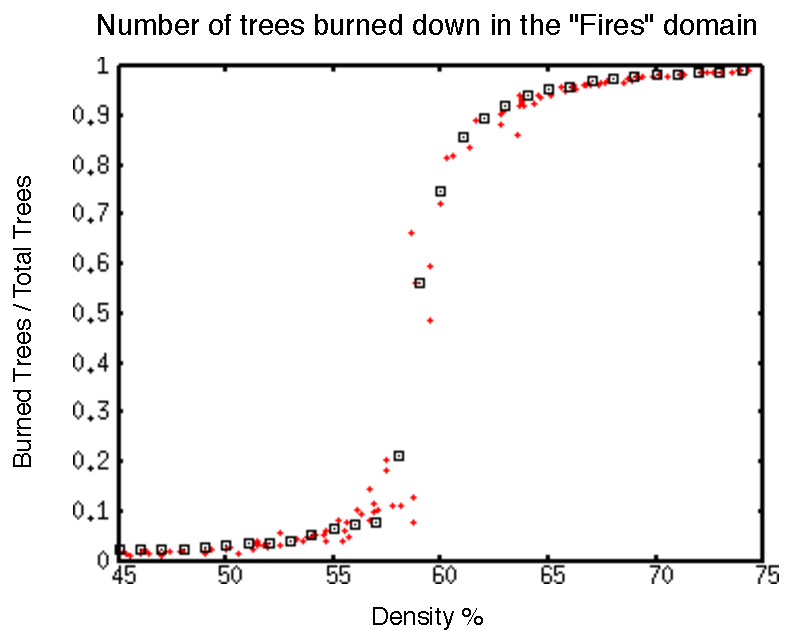
\includegraphics[scale=.5]{images/rii2.pdf}
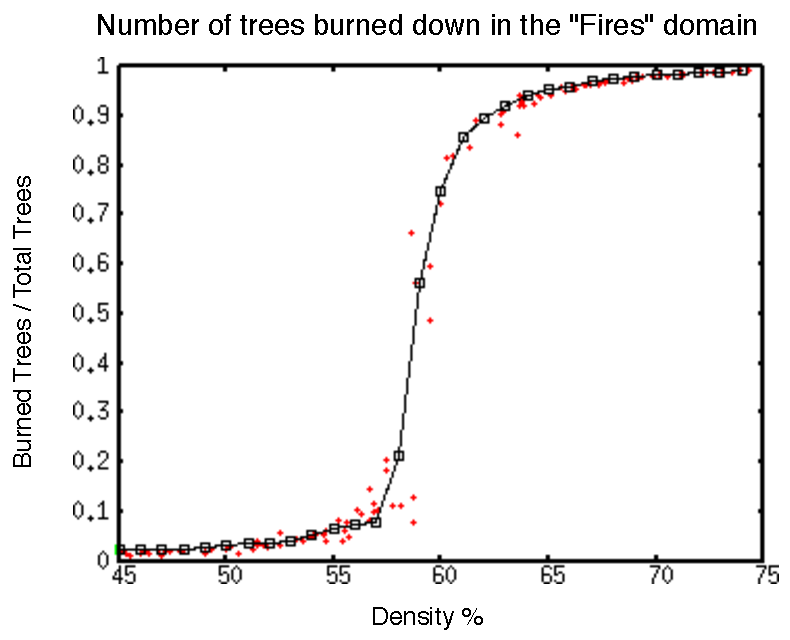
\includegraphics[scale=.5]{images/rii3.pdf}
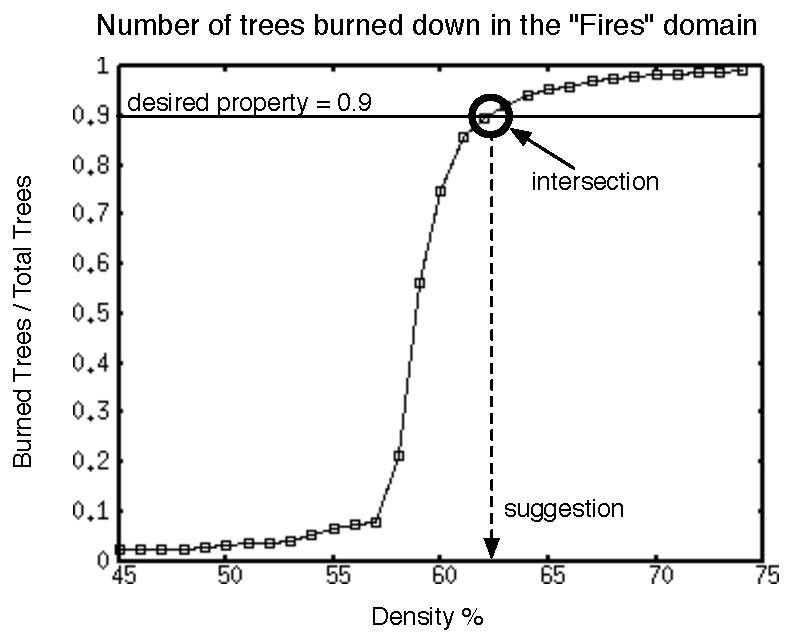
\includegraphics[scale=.5]{images/rii5.pdf}
\caption{The progression of SCI in the Fires ABM from raw data set (top left), to intersection (bottom right). }
\label{fig:rii}
\end{figure}

Next, SCI finds the intersection between the behavior space and a desired system-level property behavior $b = Burned~{ }Trees / Total~{ }Trees = 0.9$ (see bottom right image in Figure \ref{fig:rii}).
This is done by checking each simplex to see if $0.9$ is within the range of the minimum value and maximum value for $b$ in each simplex.
The only segment that intersects the $0.9$ plane is the one between 63\% and 64\%.
The intersection between this segment and the line is calculated, which in this case is approximately at $Density = 63.1$\%.

Therefore, setting $Density = 63.1$\% will be expected to yield 90\% of the trees burned down.
In higher-dimensional domains, the number of points that will satisfy the system-level property will be infinite instead of just one point, since they lie on a continuous hyperplane.

\subsection{Special Cases}

In this section, I discuss two special cases that can simplify the SCI process significantly.
Users of \fw can see significant improvements in computation time if either of these cases can be identified as a property of a domain.

   \subsubsection{Classification}
System-level properties that are binary (positive and negative) in nature (i.e., the forward-mapping is classification, not regression) can be treated differently.
SCI handles binary-valued system-level properties by labeling each simplex as either:
\begin{itemize}
\item positive -- corners are all positive instances,
\item negative -- corners are all negative instances, or
\item inconclusive -- corners are a mixture of both positive and negative instances.
\end{itemize}
Then, once a query is submitted with binary values as part of the requirement, SCI removes all simplexes that do not match that binary value.
For example, if a query contains a positive binary value, all negative and inconclusive simplexes are removed from the search.
Inconclusive simplexes are removed since there are probably a number of simplexes which will satisfy the system-level property constraint.
This is possible because these simplexes will not be part of the solution, even if other system-level properties could be satisfied by configurations within these simplexes.
This shortcut can significantly reduce computation time if a majority of the space is removed.

Inconclusive simplexes are situated on the boundary of positive and negative instances in the space.
Therefore, the granularity of the inconclusive simplexes can be increased by separating them (Subsection \ref{subsec:granularity}) in order to reduce the amount of space occupied by inconclusive simplexes.


   \subsubsection{One-to-One Mapping}
With some properties, the forward mapping may define a one-to-one mapping.
If this is the case, then regression can be used for the reverse mapping by training on the system-level property to infer values for the configuration parameters.
The regression will return the single configuration that satisfies the system-level property, since it is one-to-one.
Therefore, if a user is working with a one-to-one mapping, this should be the only property being analyzed.
Only one point is returned, so adding additional constraints will typically over specify the system of equations and not return anything.
%Even if another property's hyperplane intersects with the point, the same point will still return the same point.

The percentage of trees burned down in the Fires ABM is an example of a one-to-one relationship, since the percentage of trees burned down increases monotonically with the density of the trees.



\section{Alternative Approach I: Optimization}
In related work, researchers typically treat the problem of finding a configuration that will satisfy some system-level constraint as an optimization problem.\footnote{Section \ref{sec:invfm} summarizes related work in which researchers treat inverting the forward mapping as optimization.}
In this type of approach, an optimization meta-heuristic such as simulated annealing or genetic algorithms can be used to incrementally adjust the system configuration until the system-level properties match the final goal.
These approaches use a concept of fitness that measures the actual outcome with the expected outcome.
ABMs that exhibit closer outcomes are weighted higher so that the algorithm gradually converges on a solution.

The main reason that this approach is a poor choice for the reverse-mapping problem is that sampling the ABM on every iteration can be very slow.
To calculate the fitness of a particular configuration, the ABM must be executed and measured.
Running the Wolf Sheep Predation model takes at least one second per run.
Every generation of a genetic algorithm could have to execute an ABM several hundred times, which case, each generation could take several minutes to compute.

A hybrid approach is possible that significantly reduces the online running time of optimization.
Instead of directly sampling the ABM, the optimization technique can use the forward mapping to infer the outcome of a configuration instead of executing it.
This approach also has the benefit that the regression smooths the predictions, which in many cases will give more consistent results than querying an ABM directly.
This approach is effectively searching through the regression space created by the forward mapping, which is an approximation of the true behavior space.

\section{Alternative Approach II: Functional Inversion}\label{sec:functional}

Some regression approaches can be directly inverted.
This has the benefit that no approximation, such as SCI, has to be performed, however, a functional inversion is algorithm-dependent, meaning a new method must be implemented for each regression.

I will describe functional inversions of kNN and NLR, as examples.
kNN is conceptually and computationally difficult to invert.
The ``forward mapping" of kNN is:
What is the average of the values for the $k$ nearest points to configuration vector $\mathbf c$?
The inverse of this statement is:
What space covered by $k$ neighboring points would produce the average $p$?
One way to compute this would be to generate a structure similar to a Voronoi diagram that segregates the space into sections.
Every point within a section has the same $k$ nearest neighbors, which are iterated over to find averages that are close enough.
This search can be computationally intensive, since the number of sections can be large with relatively high values of $k$.
Also, since this space is discontinuous, finding a desired average may be impossible.
With SCI, continuous transitions are inserted between the discontinuous spaces, allowing intersections to be inferred, even if no average exists.

Nonlinear regression, on the other hand, is rather simple to invert with algebra, at least for certain parametric models.
Basically, inverting NLR reduces to satisfying the following equation:
\[f(\mathbf x, \beta) - y = 0,\]
where $\beta$ are the learned model parameters and $y$ is the desired system-level property value.
This equation can be solved with a number of numerical root finding methods.
Inverting nonlinear regression, in particular, is useful because it provides an elegant solution in the form of mathematical equations, instead of the piecewise ones provided by SCI.


\section{Using Reverse Mappings}
The main purpose of generating a reverse mapping is to gain an understanding of the space of configurations that generate a particular system-level behavior.
The relationships between configuration parameters can be inferred by analyzing these spaces.
For example, when one configuration parameter value is reduced and the other is increased by a specific amount, the resulting system-level behavior may be the same.
The equations returned by SCI provide this mathematical representation in a piecewise way.
This deeper understanding of how a system-level property can be produced is faster and potentially more valuable than having a researcher manually study a domain to gain an understanding of how the configurations affect system-level behavior.

The reverse mapping can be used to suggest a configuration when a user wishes to see a particular behavior exhibited in the ABM.
For example, suppose the user of \fw wants to determine what an execution of a Fire ABM that burns down 80\% of the trees looks like.
SCI can suggest what density of trees should be used.
Typically, the user would have to go through an iterative process of guessing a possible configuration, then executing the ABM to determine whether the configuration generated the behavior or not.
This is effectively manual hill climbing, and can be unintuitive, difficult and tedious.

To suggest a configuration with \fw, the user queries the reverse mapping with the desired system-level property values.
SCI returns the space of configurations that would satisfy this query.
Any point in this space will be satisfactory; however, the user must select one.
Whether this point is selected arbitrarily or not is up to the user.
To select an arbitrary point, a random simplex is chosen.
Then, a set of values that will satisfy the system of equations associated with that simplex are derived.
Free variables have their values randomly selected, within the range of the simplex.
The fixed variables are fixed, so their values are already given.
Together, these points provide the user with a suitable point in the solution space to configure the target ABM.

Certain points in the solution space may be considered better than others, even if they should produce similar output.
Typically, areas of the space that have minimal variance are safer choices for configuration suggestions, since the expected error is less.
As an aside, the action of removing high-variance areas of the space is possible by adding a binary-valued system-level property that separates the space into ``high-variance" and ``low-variance" spaces, given a specified threshold.
This approach has the benefit that the selection of configurations with low variance is performed inside the framework, instead of by the user.




\section{Summary}
The reverse-mapping problem is the problem of finding a one-to-many mapping that maps system-level property values to the set of ABM configurations that would exhibit that behavior.
\fw uses SCI, an approach that build an \textit{invertible} approximation of the forward mapping.
This approximated mapping can be inverted and thus return the inverse of the forward mapping.
Results detailing the computational time required offline, the computational time required per query, and the accuracy of the reverse mappings developed by \fw are discussed in the next chapter.
